\subsection{基函数回归}
\label{sec:regression-basis}

OLS、岭、SVR等都在原始输入的线性空间里拟合；真实关系弯曲时，直线会在局部系统性偏高或偏低。\term{基函数回归}（basis function regression）先把原始输入通过一组固定函数映射到新特征，再在这些新特征上作线性拟合：系数仍然是线性的，非线性来自基函数本身。

\subsubsection{模型结构}
\label{sec:regression-basis-structure}

选取基函数$\phi_j:\mathbb{R}^d\to\mathbb{R}$，预测为
\begin{equation}
  f(\bm{x})=b+\sum_{j=1}^p w_j\phi_j(\bm{x})
  =\phi(\bm{x})^{\top}\bm{w},
  \label{eq:regression-basis-model}
\end{equation}
其中$\phi(\bm{x})=(1,\phi_1(\bm{x}),\ldots,\phi_p(\bm{x}))^{\top}$。对输入可以非线性、对待估系数仍线性：基函数$\phi_j$、待学系数$w_j$、截距$b$与基函数数量$p$是不同角色，模型结构本身尚未决定损失或概率假设。增广设计矩阵$\bm{\Phi}\in\mathbb{R}^{n\times(p+1)}$的第$i$行为$\phi(\bm{x}_i)^{\top}$；把式\eqref{eq:regression-ols-objective}中的特征列换成$\bm{\Phi}$后，OLS的最小二乘目标、梯度与更新全部原样复用（待学参数变为基系数与截距）。多项式、径向基和样条是这一扩展的具体表示，下面分别展开。

\subsubsection{参数学习}
\label{sec:regression-basis-learning}

采用平均半平方目标$J=(2n)^{-1}\sum_i e_i^2$，其中$e_i=f(\bm{x}_i)-y_i$；用链式法则给出$\partial J/\partial w_j=n^{-1}\sum_i e_i\phi_j(\bm{x}_i)$与$\partial J/\partial b=n^{-1}\sum_i e_i$，同一轮误差下同步更新。增广设计的直接最小二乘求解为$\bm{\Phi}^{\top}\bm{\Phi}\widehat{\bm{w}}=\bm{\Phi}^{\top}\bm{y}$；高阶多项式列之间高度相关，$\bm{\Phi}^{\top}\bm{\Phi}$条件数很大，可对基列中心化、正交化（如QR）或加入岭惩罚后求解。训练与预测沿用同一特征变换、中心和尺度；基函数中心或尺度也学习时，需另外求相应导数，不能继续当成固定设计线性求解。基参数（RBF中心与半径、样条节点）通常先固定，再与基数量一起由训练内验证选择；新输入按同一组基计算$\phi(\bm{x}_\star)$，中心、半径、节点不得用测试数据调整，数值上避免直接求逆，秩亏时取最小范数解。

\subsubsection{多项式展开：增加曲率与交互}
\label{sec:regression-basis-polynomial}

\paragraph{多项式模型与系数学习}

$b+w_1x$无法表示斜率随输入改变的关系，局限来自特征表示，平方损失仍可使用。以$m(x)=x^2$为教学例，明确写出新模型$f(x)=b+w_1x+w_2x^2+\cdots+w_qx^q$，次数$q$是待选配置，$b,w_1,\ldots,w_q$是待学系数，对应设计行是$(1,x,\ldots,x^q)$。把一般梯度中的基函数换为$x_i^j$，即$\partial J/\partial w_j=n^{-1}\sum_i e_i x_i^j$，扩大设计后直接求解，不再重讲梯度下降的一般原理。

图\ref{fig:regression-feature-approximation}中，在$(2,4)$两个样本上拟合$x^2$，最佳直线解为$y=0.5x+1$——直线在两点间近似抛物线，但没有$x^2$项时无法复现曲率；这一结果区分候选空间的表示误差与有限数据的训练、预测误差，为次数选择建立比较对象。

\begin{figure}[htbp]
  \centering
  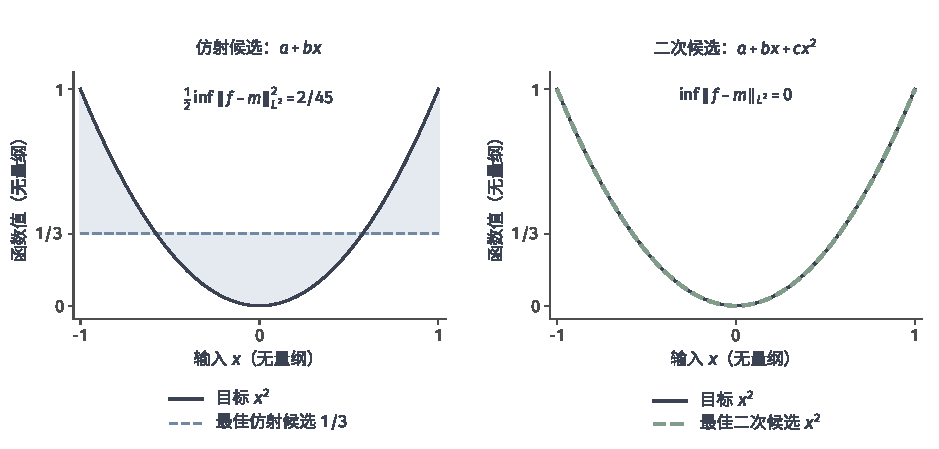
\includegraphics[width=105.412mm]{figures/04-classic-models/00-shared/matplotlib/regression-feature-approximation/figure.pdf}
  \caption{两个样本上的线性近似。虚线为目标$x^2$，蓝点为$(2,4)$，实线为最小二乘直线$y=0.5x+1$。两点上精确拟合，区间外偏差随距离增大；增加$x^2$基才能在训练点上复现抛物线曲率。}
  \label{fig:regression-feature-approximation}
\end{figure}

将单变量推广到多个输入时，以$x_1x_2$说明一个变量的作用可以随另一个变量改变。用多重指标$\bm{a}$与总次数$|\bm{a}|=\sum_ja_j$定义非恒定单项式$\bm{x}^{\bm{a}}=\prod_jx_j^{a_j}$，选$1\le|\bm{a}|\le q$形成设计列，$f(\bm{x})=b+\sum_{1\le|\bm{a}|\le q}w_{\bm{a}}\bm{x}^{\bm{a}}$，$\partial J/\partial w_{\bm{a}}=n^{-1}\sum_i e_i\bm{x}_i^{\bm{a}}$；交互项与单变量高次项的区别在此明确。

\paragraph{次数选择与外推}

比较嵌套的多项式空间，增加次数使最佳训练误差不增，却不能推出测试误差下降；多变量下增加总次数还会增加候选单项式数量，需要同时考虑样本与计算规模。因此在训练折构造特征并拟合，在验证折比较次数与正则强度。高次幂会带来数值放大，样本之外按最高次项发散，不能因训练区间内拟合改善就把结论外推到区间外。

\subsubsection{径向基与样条：表达局部变化}
\label{sec:regression-basis-local}

\paragraph{径向基函数}

高次多项式影响整个区间，于是另一种思路是只在某些位置改变曲线，统一写$f(x)=b+\sum_jw_j\phi_j(x)$。\term{径向基}（RBF）取$\phi_j(\bm{x})=\exp(-\lVert\bm{x}-\bm{c}_j\rVert_2^2/(2r_j^2))$，每个中心$\bm{c}_j$只在附近隆起，组合后局部覆盖；中心$\bm{c}_j$与宽度$r_j$先固定，构建设计矩阵$\Phi_{ij}=\phi_j(\bm{x}_i)$后权重梯度把前节的$x_i^j$换成$\phi_j(\bm{x}_i)$，截距梯度不变。中心和宽度的选择只用训练数据及验证。

\paragraph{样条的接合与表示}

与径向基的局部衰减对照，\term{样条基}把输入分段，在每段内用低次多项式、段间施加连续导数条件。以三次样条为例，设内部结点为$\xi_1<\cdots<\xi_K$，截断幂基取为
\[
  f(x)=\beta_0+\beta_1 x+\sum_{k=1}^K\gamma_k\,(x-\xi_k)_+^3,
\]
其中$(x-\xi_k)_+^3=\max(0,x-\xi_k)^3$。在结点$\xi_k$左侧，该项为零；右侧为$(x-\xi_k)^3$。检查结点左右：函数值从$0$到$0$连续，一阶导数$3(x-\xi_k)^2$两侧都为零，二阶导数$6(x-\xi_k)$两侧都为零，只有三阶导数从$0$跳到$6\gamma_k$。因此$f$、$f'$、$f''$在每个结点处连续，整条曲线二阶光滑，三阶导数在结点处允许跳跃——这正是三次样条的接合条件。把$(1,x,(x-\xi_1)_+^3,\ldots,(x-\xi_K)_+^3)$作为基列构建设计矩阵，系数$\beta_0,\beta_1,\gamma_k$仍由普通最小二乘或加岭惩罚拟合。截断幂基整体平滑但支撑遍及全域，数值条件较差；实际计算常用\term{B样条基}，它在每个结点区间上由少量邻近基函数组合而成、支撑局部化，描述的是同一个三次样条空间，只是基条件数更好。更换基后，训练与预测必须使用同一组基函数，基的结点位置由训练数据或验证选定，不在新输入上重排。

\paragraph{表示选择与配置}

三种表示职责不同：多项式基影响全局、次数决定曲率；RBF在中心附近局部隆起；样条在结点附近弯曲、段间由导数条件保证光滑。基数量增加意味着待估系数增多、估计方差上升，需要更多数据支撑；固定基不学习非线性参数，基的位置与形状本身是结构假设，选错基时系数再小也补不回来。多项式在训练区间之外按最高次项发散，外推不可靠；RBF在远离中心处归零，局部平滑但覆盖范围有限。选择应匹配任务在训练域内、外的要求，平滑惩罚由GAM进一步展开。
